% This is "sig-alternate.tex" V2.0 May 2012
% This file should be compiled with V2.5 of "sig-alternate.cls" May 2012
%
% This example file demonstrates the use of the 'sig-alternate.cls'
% V2.5 LaTeX2e document class file. It is for those submitting
% articles tol ACM Conference Proceedings WHO DO NOT WISH TO
% STRICTLY ADHERE TO THE SIGS (PUBS-BOARD-ENDORSED) STYLE.
% The 'sig-alternate.cls' file will produce a similar-looking,
% albeit, 'tighter' paper resulting in, invariably, fewer pages.
%
% ----------------------------------------------------------------------------------------------------------------
% This .tex file (and associated .cls V2.5) produces:
%       1) The Permission Statement
%       2) The Conference (location) Info information
%       3) The Copyright Linle with ACM data
%       4) NO page numbers
%
% as against the acm_proc_article-sp.cls file which
% DOES NOT produce 1) thru' 3) above.
%
% Using 'sig-alternate.cls' you have control, however, from within
% the source .tex file, over both the CopyrightYear
% (defaulted to 200X) and the ACM Copyright Data
% (defaulted to X-XXXXX-XX-X/XX/XX).
% e.g.
% \CopyrightYear{2007} will cause 2007 to appear in the copyright line.
% \crdata{0-12345-67-8/90/12} will cause 0-12345-67-8/90/12 to appear in the copyright line.
%
% ---------------------------------------------------------------------------------------------------------------
% This .tex source is an example which *does* use
% the .bib file (from which the .bbl file % is produced).
% REMEMBER HOWEVER: After having produced the .bbl file,
% and prior to final submission, you *NEED* to 'insert'
% your .bbl file into your source .tex file so as to provide
% ONE 'self-contained' source file.
%
% ================= IF YOU HAVE QUESTIONS =======================
% Questions regarding the SIGS styles, SIGS policies and
% procedures, Conferences etc. should be sent to
% Adrienne Griscti (griscti@acm.org)
%
% Technical questions _only_ to
% Gerald Murray (murray@hq.acm.org)
% ===============================================================
%
% For tracking purposes - this is V2.0 - May 2012

\documentclass{sig-alternate-2013}

\usepackage{subfigure}
\usepackage{epsfig}
\usepackage[ruled]{algorithm2e}
\usepackage{algorithmic}

\newfont{\mycrnotice}{ptmr8t at 7pt}
\newfont{\myconfname}{ptmri8t at 7pt}
\let\crnotice\mycrnotice%
\let\confname\myconfname%

\permission{Permission to make digital or hard copies of all or part of this work for personal or classroom use is granted without fee provided that copies are not made or distributed for profit or commercial advantage and that copies bear this notice and the full citation on the first page. Copyrights for components of this work owned by others than ACM must be honored. Abstracting with credit is permitted. To copy otherwise, or republish, to post on servers or to redistribute to lists, requires prior specific permission and/or a fee. Request permissions from permissions@acm.org.}
\conferenceinfo{MM'14,}{November 03 - 07 2014, Orlando, FL, USA.}
\copyrightetc{Copyright 2014 ACM \the\acmcopyr}
\crdata{978-1-4503-3063-3/14/11\ ...\$15.00.\\
http://dx.doi.org/10.1145/2647868.2654905}

\clubpenalty=10000
\widowpenalty = 10000

\begin{document}
%
% --- Author Metadata here ---
%\conferenceinfo{WOODSTOCK}{'97 El Paso, Texas USA}
%\CopyrightYear{2007} % Allows default copyright year (20XX) to be over-ridden - IF NEED BE.
%\crdata{0-12345-67-8/90/01}  % Allows default copyright data (0-89791-88-6/97/05) to be over-ridden - IF NEED BE.
% --- End of Author Metadata ---

\title{Social Embedding Image Distance Learning}

%
% You need the command \numberofauthors to handle the 'placement
% and alignment' of the authors beneath the title.
%
% For aesthetic reasons, we recommend 'three authors at a time'
% i.e. three 'name/affiliation blocks' be placed beneath the title.
%
% NOTE: You are NOT restricted in how many 'rows' of
% "name/affiliations" may appear. We just ask that you restrict
% the number of 'columns' to three.
%
% Because of the available 'opening page real-estate'
% we ask you to refrain from putting more than six authors
% (two rows with three columns) beneath the article title.
% More than six makes the first-page appear very cluttered indeed.
%
% Use the \alignauthor commands to handle the names
% and affiliations for an 'aesthetic maximum' of six authors.
% Add names, affiliations, addresses for
% the seventh etc. author(s) as the argument for the
% \additionalauthors command.
% These 'additional authors' will be output/set for you
% without further effort on your part as the last section in
% the body of your article BEFORE References or any Appendices.
\numberofauthors{1} %  in this sample file, there are a *total*
% of EIGHT authors. SIX appear on the 'first-page' (for formatting
% reasons) and the remaining two appear in the \additionalauthors section.
%
\author{
% You can go ahead and credit any number of authors here,
% e.g. one 'row of three' or two rows (consisting of one row of three
% and a second row of one, two or three).
%
% The command \alignauthor (no curly braces needed) should
% precede each author name, affiliation/snail-mail address and
% e-mail address. Additionally, tag each line of
% affiliation/address with \affaddr, and tag the
% e-mail address with \email.
%
% 1st. author
\alignauthor
Shaowei Liu${}^1$, Peng Cui${}^1$, Wenwu Zhu${}^1$, Shiqiang Yang${}^1$ and Qi Tian${}^2$\\
\affaddr{${}^1$Computer Science Department, Tsinghua University, China}\\
\affaddr{${}^2$Department of Computer Science, University of Texas at San Antonio}\\
\small{\email{liu-sw11@mails.tsinghua.edu.cn, cuip/wwzhu/yangshq@tsinghua.edu.cn,  qitian@cs.utsa.edu}}
% 2nd. author
%\alignauthor
%G.K.M. Tobin\titlenote{The secretary disavows
%any knowledge of this author's actions.}\\
%       \affaddr{Institute for Clarity in Documentation}\\
%       \affaddr{P.O. Box 1212}\\
%       \affaddr{Dublin, Ohio 43017-6221}\\
%       \email{webmaster@marysville-ohio.com}
%% 3rd. author
%\alignauthor Lars Th{\o}rv{\"a}ld\titlenote{This author is the
%one who did all the really hard work.}\\
%       \affaddr{The Th{\o}rv{\"a}ld Group}\\
%       \affaddr{1 Th{\o}rv{\"a}ld Circle}\\
%       \affaddr{Hekla, Iceland}\\
%       \email{larst@affiliation.org}
%\and  % use '\and' if you need 'another row' of author names
%% 4th. author
%\alignauthor Lawrence P. Leipuner\\
%       \affaddr{Brookhaven Laboratories}\\
%       \affaddr{Brookhaven National Lab}\\
%       \affaddr{P.O. Box 5000}\\
%       \email{lleipuner@researchlabs.org}
%% 5th. author
%\alignauthor Sean Fogarty\\
%       \affaddr{NASA Ames Research Center}\\
%       \affaddr{Moffett Field}\\
%       \affaddr{California 94035}\\
%       \email{fogartys@amesres.org}
%% 6th. author
%\alignauthor Charles Palmer\\
%       \affaddr{Palmer Research Laboratories}\\
%       \affaddr{8600 Datapoint Drive}\\
%       \affaddr{San Antonio, Texas 78229}\\
%       \email{cpalmer@prl.com}
}
% There's nothing stopping you putting the seventh, eighth, etc.
% author on the opening page (as the 'third row') but we ask,
% for aesthetic reasons that you place these 'additional authors'
% in the \additional authors block, viz.
%\additionalauthors{Additional authors: John Smith (The Th{\o}rv{\"a}ld Group,
%email: {\texttt{jsmith@affiliation.org}}) and Julius P.~Kumquat
%(The Kumquat Consortium, email: {\texttt{jpkumquat@consortium.net}}).}
% Just remember to make sure that the TOTAL number of authors
% is the number that will appear on the first page PLUS the
% number that will appear in the \additionalauthors section.

\maketitle

\input{Abstract}

% A category with the (minimum) three r equired fields
\category{H.3.3}{Information Search and Retrieval}{Retrieval models}

\terms{Algorithms, Experimentation, Performance}

\keywords{image search and recommendation, social similarity, user behavior, metric learning}

\vspace{-0.3cm}\section{INTRODUCTION}
With the fast development of Internet, images play an important role in delivering information in our daily life. Thus, understanding images become an increasing demand. In image processing and understanding applications, such as image search, recommendation and classification, measuring the distance (or similarity) of pair-wise images is a fundamental and important issue. \emph{If an effective image distance metric is obtained, we can easily employ existing technologies to achieve satisfactory performance in such applications\cite{visualrank,cbf}.}

However, to date, existing image distance metrics do not perform well to achieve this goal, due to the fact that they usually focus on measuring similarity of visual features but are not mature to capture user intention, especially in human related applications, such as image search and recommendation. Here user intention includes many aspects, such as semantics, attributes, emotion, layout, etc. Although the problem of capturing user intention has received increasing attention, how to identify and understand it is still a great challenge because there is a huge gap between level visual contents and high level user intention, which is called intention gap.

 With the development of social network, a huge amount of users share their beautiful pictures and view others' in the social media platforms, such as Flickr and Twitter. Within these platforms, we can obtain not only vast amounts of images but also a series of collective social and behavioral information, such as annotated tags, favorite images and interest groups of users. In social psychology, it has been proved that human cognition and user behavior influence each other \cite{cognitive}. Therefore, social behavioral information in social media platform can be regarded as the reflection of their intention when viewing images. Given user behavior information in the social media platforms, we can use to better evaluate image distance. In recent years, there are some works that focus on using social information to better evaluate image similarity and achieves some improvements. However, they are limited due to the following challenges:


 %Although the technologies up to date can hardly estimate the user cognition behind his behavior, we can easily evaluate the similarity of user behaviors of two images. For a pair of images, if users have similar behaviors (such as favoring, sharing and tagging), their cognition to the images would also be similar. In this paper, we refer to the similarity of users' social behaviors as social similarity.



(1) \textbf{The lack of social information in general Web image.} Although behavioral information does help to estimate user cognition, most of the Web images do not have user behavior information due to the fact that they are not produced by social media platforms. If the image distance relies on  social behavioral data, our method will be extremely circumscribed in social images. Therefore, how to make our distance metric universal in common Web images is a great challenge in our problem.

(2) \textbf{The unreliability and sparsity of social media data.} In social network, collective social and behavioral information is usually sparse and unreliable. If the amount of user behavior information is not enough, the social similarity may have contingency. Not all of image pairs's social similarity can be evaluated well. Thus, we also need to consider the reliability of social similarity and balance the social similarity and visual similarity in this case.

(3) \textbf{The sparsity of user behavior.} 


%(3) The Heterogeneity of social data. Different with traditional homogeneous data structure, the data in social media is heterogeneous  and hybrid. For example, a user may publish and favor a lot of images and an image may be shared to a series of interest groups. Therefore, to make our method extensible, we should formulate these multi-modal information in a unified structure.

\begin{figure*}
\centering
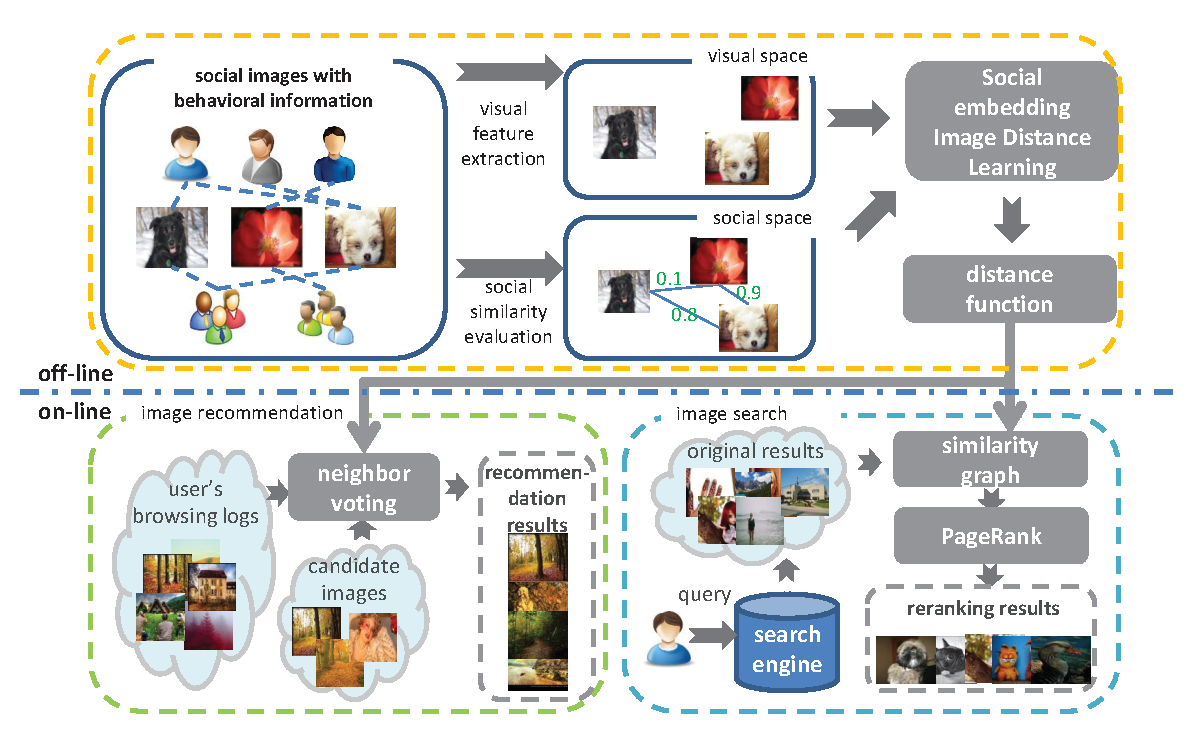
\epsfig{file=framework.eps, width = 5.2in, height = 2.4in}
\caption{Illustration of the proposed Social embedding Image Distance Learning (\emph{SIDL}) approach and the image search and recommendation system developed on \emph{SIDL}.}
\label{framework}
\end{figure*}

To address the above problems, we propose a Social embedding Image Distance Learning (\emph{SIDL}) approach to learn image distance from user behavior information in social media platforms, which is shown in Figure \ref{framework}. In the approach, we use metric learning technique to learn an image distance function of visual features. Different from traditional metric learning work, our distance function aims at making image distance consistent to their social distance in user behavior. Thus, although the distance function is learned from social images (i.e., the images in social media platforms), it can measure the distance of ordinary Web images because it learns the weight and correlation of visual features. We call this idea ``learn from social image, work beyond social image". In our method, we first estimate the social similarity among social images, where the reliability of social entities is evaluated. Next, we conduct our metric learning method to reduce the distance of socially similar images and enlarge the distance of socially dissimilar images. Finally, the learned image distance function is used to evaluate the distance of Web images based on their visual features. The image distance can be applied to a lot of applications, such as image recommendation and reranking. We not only conduct comprehensive experiments to show the effectiveness of our approach, but also give an interesting observation about the relationship between the learned distance and our intuitive cognition.

The contributions of our proposed approach are summarized as follows:

(1) We propose a novel image distance learning approach, which aims at using user behavior information in social media to capture human cognition in Web image distance measuring. To the best of our knowledge, we are the first who use the idea of ``learn from social media, work beyond social media" to solve this problem.

(2) In this paper, we propose a Social Embedding Image Distance Learning approach, where an image distance metric function based on visual features is learned to make image distance consistent to social distance defined from user behavior. In our approach, social distance is well estimated in multimodal social factors. The metric learning method is especially designed to learn the similarity of visual features from social distance. Furthermore, we design two basic application scenarios based on the proposed \emph{SIDL} method, including image recommendation and image reranking.

(3) To evaluate the performance of our approach, comprehensive experiments are conducted based on real social media and image reranking datasets. The experimental results have shown the effectiveness of the learning method. In addition, compared to the state-of-the-art image distance metrics the superiority of our image distance metric in the applications of image recommendation and reranking is also demonstrated.

(4) More than quantitative evaluation, an interesting observation of the relationship between the learned distance and our intuitive cognition is also given to show our results subjectively. We can observe that the key points of images, such as eyes, salient objects, are more important in measuring image similarity.

The rest of the paper is organized as follows: Section 2 gives a brief overview and comparison of related work. Section 3 introduces the evaluation of image social similarity. In Section 4, we introduce optimization of the proposed \emph{SIDL} method and present two applications including image reranking and recommendation based on our distance learning method. Then, we introduce our experiments and report the results in Section 5. Finally, Section 6 summarizes the paper.

\input{Related}
\input{Model}
\input{Applications}
\input{Experiments}
\input{Conclusion}
\vspace{-0.3cm}\section{ACKNOWLEDGEMENT}
This work was supported by National Natural Science Foundation of China, No. 61370022, No.
61303075 and No. 61210008; International Science and Technology Cooperation Program of China,
No. 2013DFG12870; National Program on Key Basic Research Project, No. 2011CB302206.
 This work was also supported in part to Dr. Qi Tian by ARO grant W911NF-12-1-0057, Faculty Research Award by NEC Laboratories of America, respectively. This work was supported in part by NSFC 61128007.Thanks for the support of NExT Research Center funded by MDA, Singapore, under the research
grant, WBS:R-252-300-001-490.

\bibliographystyle{abbrv}
\small
\bibliography{sigproc}

\end{document}
